\vspace{-20pt}
\section{Procedure}
\label{sec:Procedure}

The first step is to find the minimal current value for the laser setup, where
it is still lasing. For this measurement the setup is changed to the configuration shown in
figure~\ref{fig:setup_current}. A voltmeter is connected to the laser current
monitor for a precise voltage measurement. It has a resistance
of $\SI{100}{\ohm}$.
The minimum can be found in an iterative procedure, which follows the following
steps. First pick a current, where the laser is lasing.
Then lower the current slightly below the lasing threshold and try to bring the system back to lasing,
by adjusting the cavity with the two knobs.
If this is possible, lower the current
until it is slightly below the threshold and repeat the procedure.

\begin{figure}
  \vspace{-10pt}
  \centering
  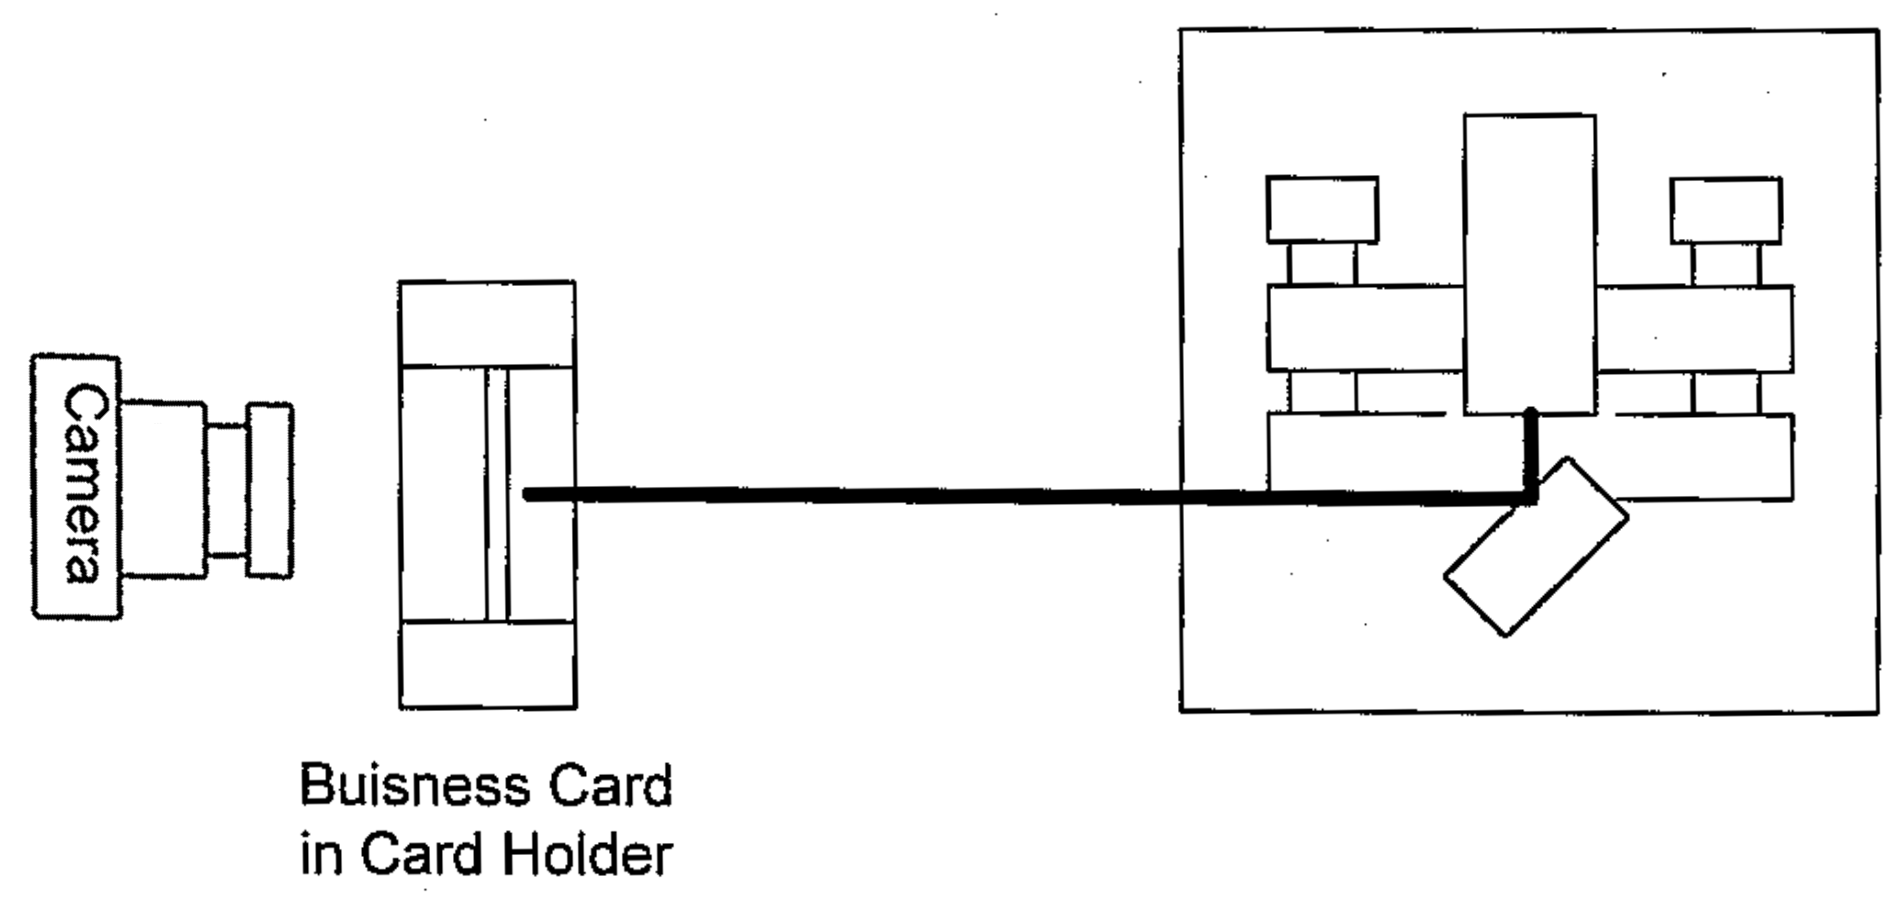
\includegraphics[width=0.75\textwidth]{Pics/setup_threshold.png}
  \caption{Setup for the minimum current measurement.\cite{anleitung}}
  \label{fig:setup_current}
\end{figure}

The minimun current below the threshold $I_{below}$ and the current above the treshold $I_{above}$
are given in~\eqref{eqn:nolase} and~\eqref{eqn:lase}.
The associated images of the laser spots are shown in figure~\ref{fig:no_lase}
and~\ref{fig:lase}.
\vspace{-10pt}
\begin{align}
  \label{eqn:nolase}
  I_{below} &= \SI{33.2}{\milli\ampere}\\
  \label{eqn:lase}
  I_{above} &= \SI{33.4}{\milli\ampere}
\end{align}

\begin{figure}[h!]
  \centering
  \begin{subfigure}{0.48\textwidth}
    \centering
    \includegraphics[width=\textwidth]{Pics/threshold_no_lase.jpg}
    \caption{Current below threshold $I_{below}$.}
    \label{fig:no_lase}
  \end{subfigure}
  \begin{subfigure}{0.48\textwidth}
    \centering
    \includegraphics[width=\textwidth]{Pics/threshold_lase.jpg}
    \caption{Current above threshold $I_{above}$.}
    \label{fig:lase}
  \end{subfigure}
\end{figure}
\FloatBarrier

The setup is now changed to the configuration shown in figure~\ref{fig:setup_fluorescence},
so that the image depicted in~\ref{fig:fluorescence} can be taken. The image
shows the Rubidium fluorescence in the gas chamber.

\begin{figure}
  \centering
  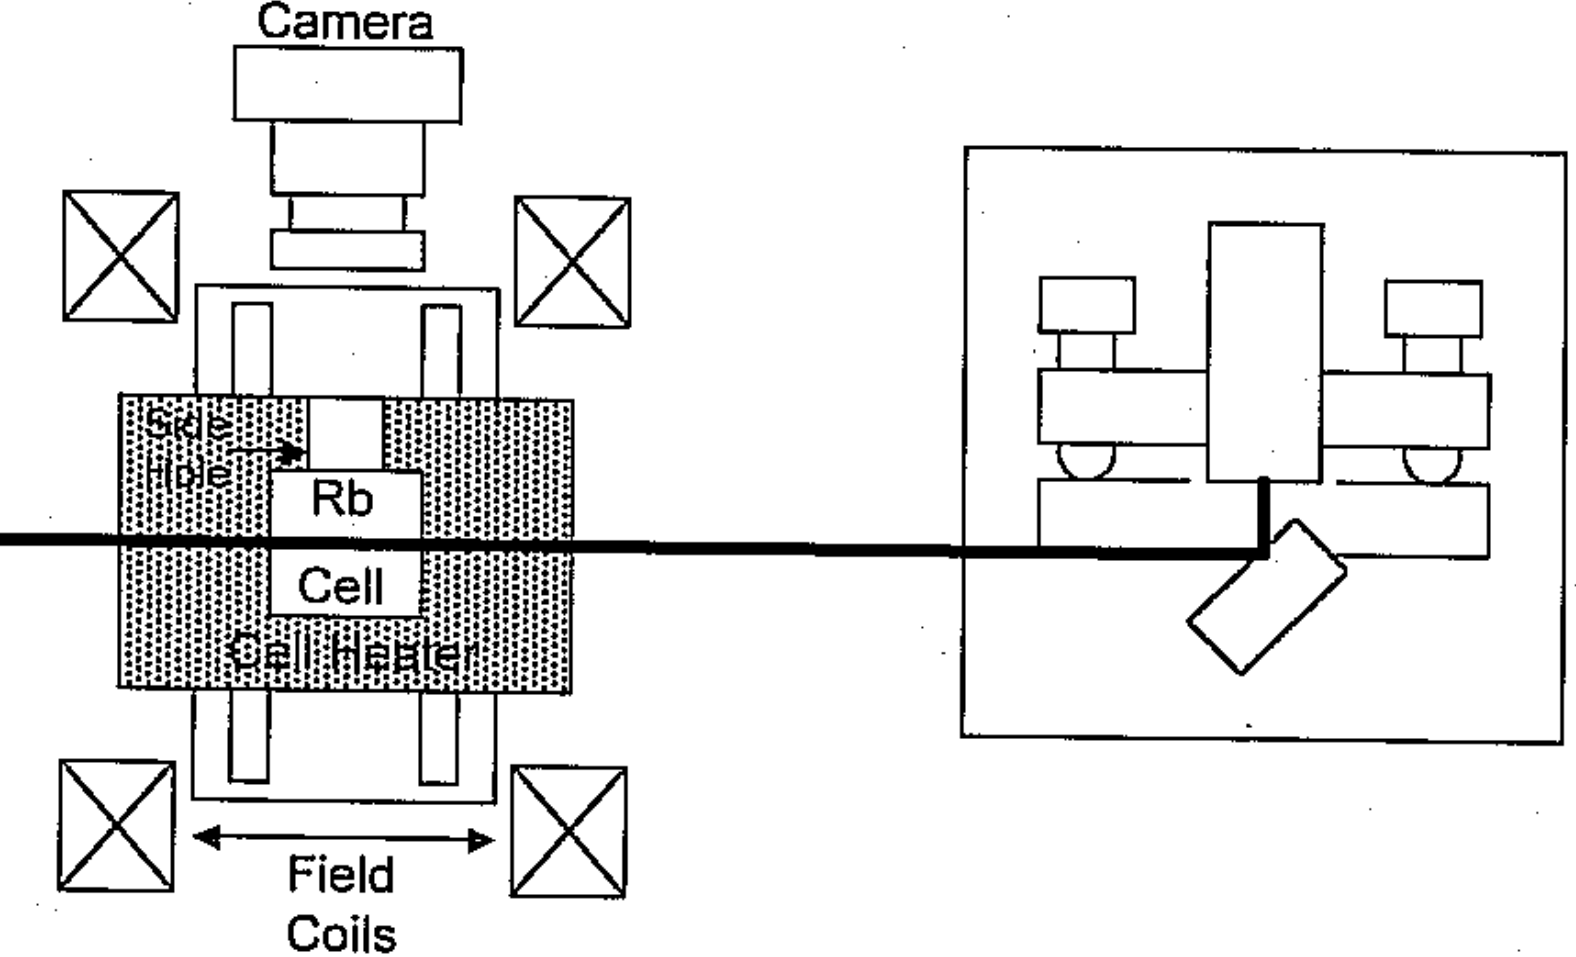
\includegraphics[width=0.8\textwidth]{Pics/setup_fluorescence.png}
  \caption{Setup to observe the Rubidium fluorescence line.\cite{anleitung}}
  \label{fig:setup_fluorescence}
\end{figure}

\begin{figure}
  \centering
  \includegraphics[width=0.5\textwidth]{Pics/Rb_fluorescence.jpg}
  \caption{Rubidium fluorescence line.}
  \label{fig:fluorescence}
\end{figure}

\FloatBarrier
Now the setup shown in figure~\ref{fig:setup_spectrum} is built up.
The current applied to the piezo is connected to an oscilloscope
for the following measurements. The piezo current is sweeped with a rectangular
voltage, so that the wavelength of the laser gets tuned over a broad spectrum.
Furthermore the current emmited by the photo diode is similary connected to the oscilloscope.

Figure~\ref{fig:example} shows an example spectrum for Rubidium. Whenever
the laser beam has the right energy to excite an Rubidium atom, the
measured intensity drops to a minimum. Figure~\ref{fig:example} contains
mode hops, which lead to an imprecise spectrum.
Therefore the setup is slightly changed. The internal cavity and the external cavity
are now varied simultaneously, which prevent mode hops.
Now the Rubidium spectrum can be measured precise. The observed spectrum
is shown in figure~\ref{fig:spectrum}. The identification of the Rubidium isotopes
is made by the comparison with reference~\cite{anleitung}.
This setup effects that there is a linear backgroud through the variation
of the laser current.

\begin{figure}
  \centering
  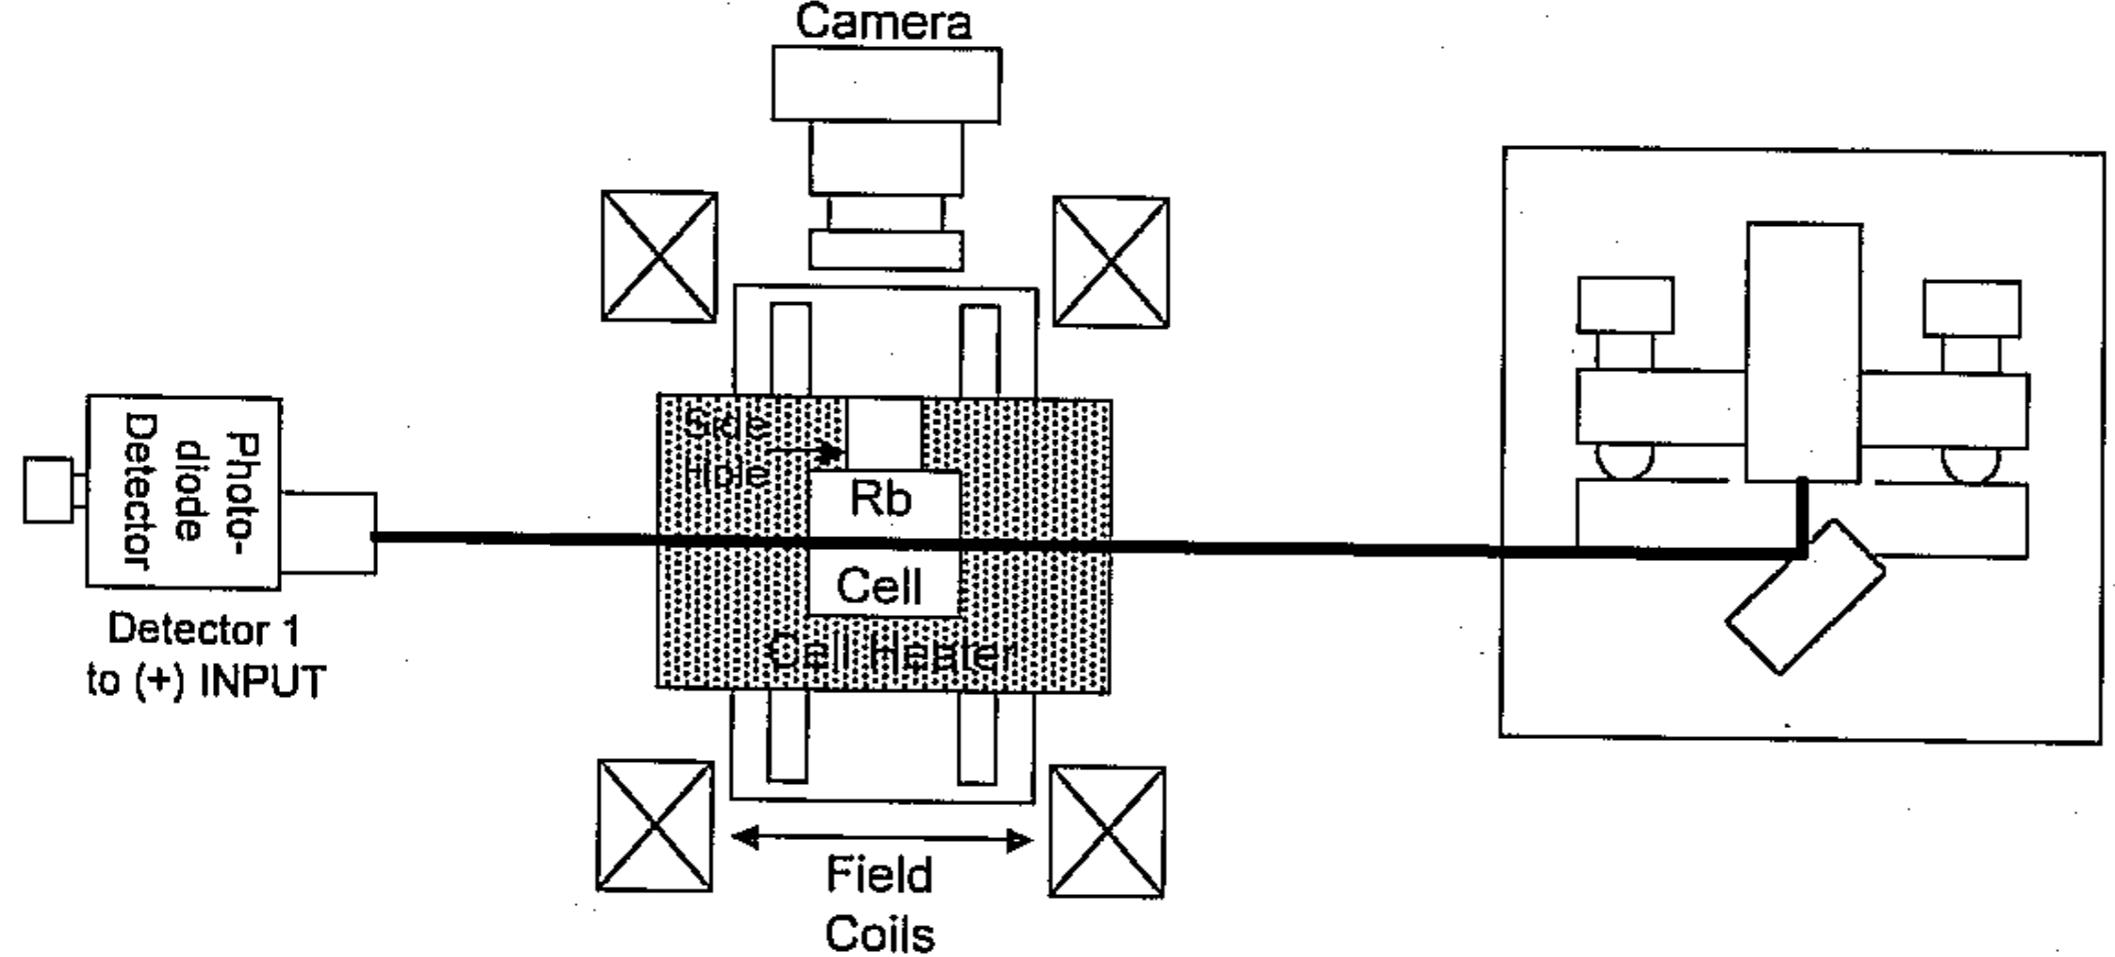
\includegraphics[width=0.8\textwidth]{Pics/setup_spectrum.png}
  \caption{Setup for the Rubidium spectrum measurement.\cite{anleitung}}
  \label{fig:setup_spectrum}
\end{figure}

\begin{figure}
  \centering
  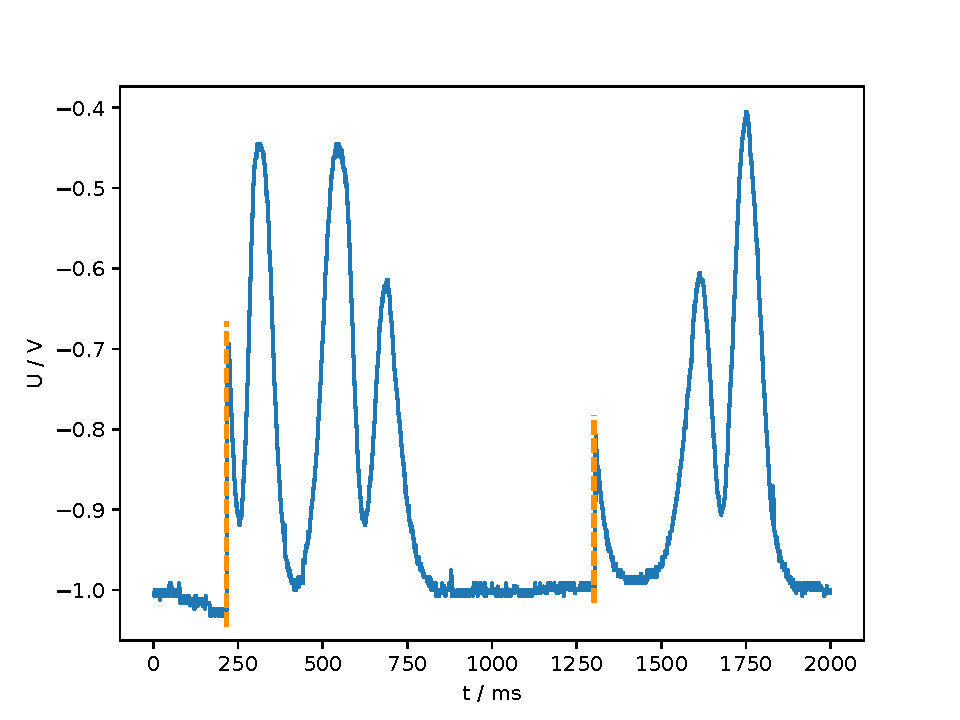
\includegraphics[width=0.7\textwidth]{Pics/example_spectrum_hop.pdf}
  \caption{Example Rubidium spectrum. The mode hopes are indicated by the orange markers.}
  \label{fig:example}
\end{figure}

\FloatBarrier
\begin{figure}
  \centering
  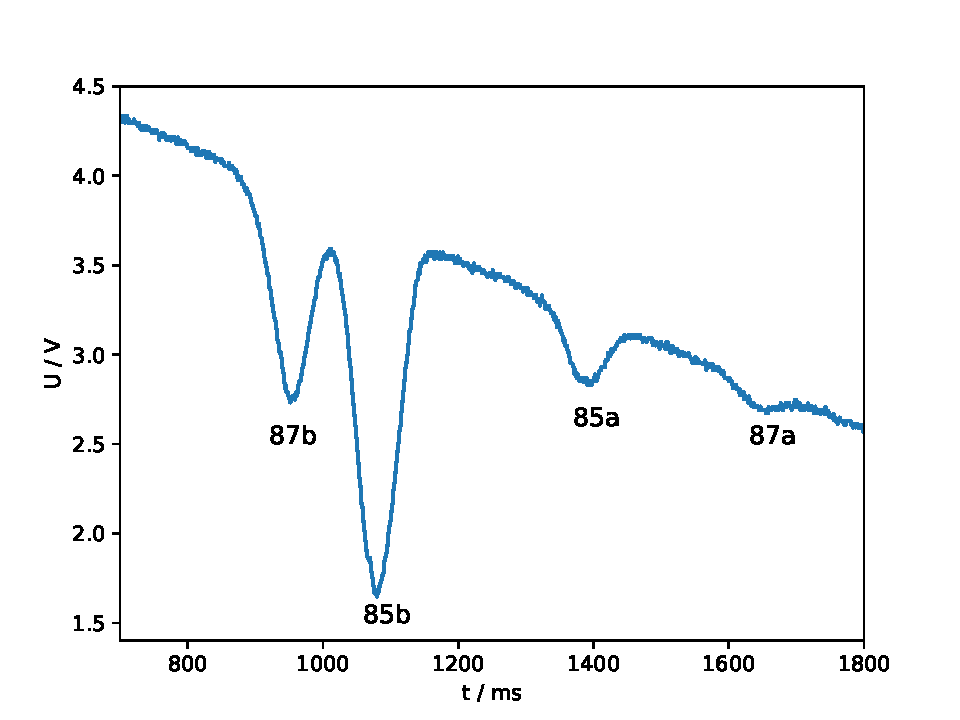
\includegraphics[width=0.7\textwidth]{Pics/Rb_spectrum.pdf}
  \caption{Rubidium spectrum.}
  \label{fig:spectrum}
\end{figure}
\FloatBarrier

The linear background in figure~\ref{fig:spectrum} can be suppressed by the
setup shown in image~\ref{fig:setup_substraction}.
This technique is called substraction technique.
The resulting spectrum is shown in figure~\ref{fig:spectrum_sub}.

\begin{figure}
  \centering
  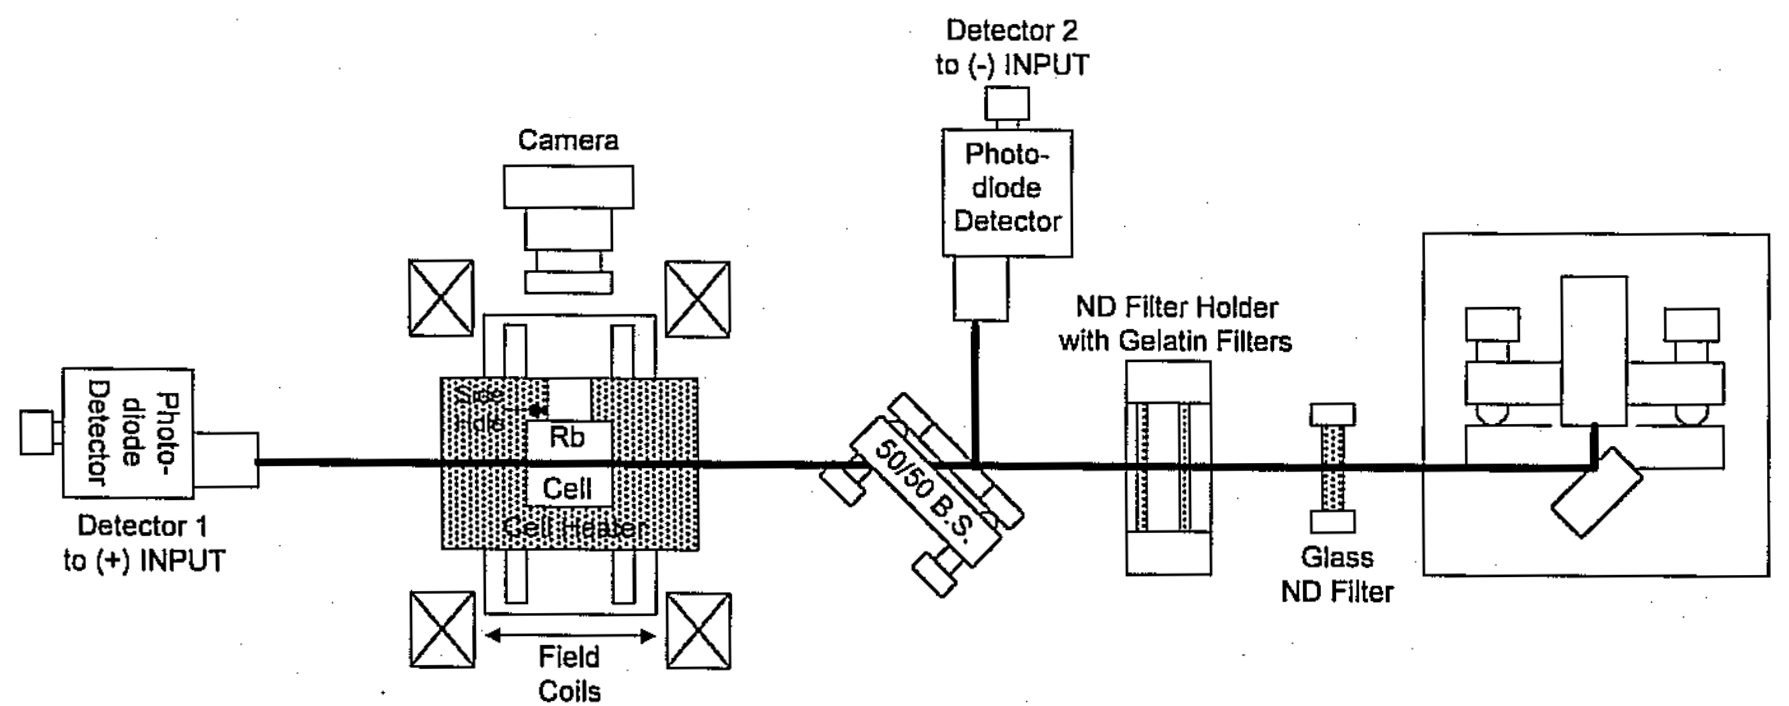
\includegraphics[width=\textwidth]{Pics/setup_substraction.png}
  \caption{Setup for the substraction technique measurement.\cite{anleitung}}
  \label{fig:setup_substraction}
\end{figure}


\begin{figure}
  \centering
  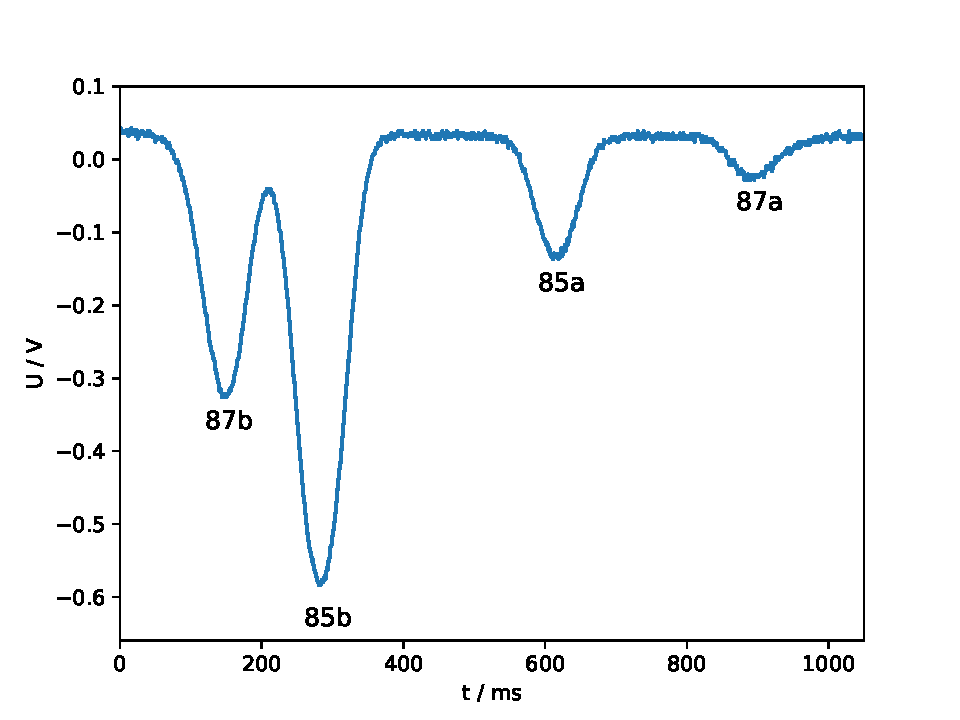
\includegraphics[width=0.7\textwidth]{Pics/Rb_spectrum_subst.pdf}
  \caption{Rubidium spectrum with substraction technique.}
  \label{fig:spectrum_sub}
\end{figure}
